\section{Considerações Iniciais}

Como apresentado no Capítulo~\ref{chapter:adm_kdm} o metamodelo KDM é capaz de agrupar diferentes visões/artefatos de um determinado sistema em uma única instância, bem como representar todas as dependências entre tais visões/artefatos. Usualmente, o que é encontrado na literatura (colocar refs) durante o desenvolvimento e manutenção de software seguindo as diretrizes e passos da abordagem MDE, é que o software geralmente é modelado e representado utilizando diferentes instâncias de metamodelos para representar as visões e todos os artefatos de um sistema. Em outras palavras, geralmente existem metamodelos para abstrair e representar o código-fonte, metamodelos para representar e abstrair o banco de dados, metamodelos para representar e abstrair a arquitetura do sistema, etc. 

Uma premissa fundamental é manter todas as instâncias dos metamodelos que representam as visões/artefatos sincronizados durante todo o processo de modernização do software. Dessa forma, quando as visões/artefatos representados em nível de modelos são alterados, é de extrema importância realizar um conjunto de propagação de mudança por todas as visões/artefatos para mantê-los atualizados e sincronizados, espelhando assim, a alteração em todas as visões/artefatos do software. Usualmente, como apresentado nos Capítulo~\ref{chapter:fundamentacao_teorica}, Seção~\ref{sec:refatoracao} e Capítulo~\ref{chapter:catalogo_refactoring_KDM} essas alterações podem ser realizadas por meio de refatorações, as quais são atividades centrais durante o processo de modernização (ref). Porém, quando um software é representado utilizando diferentes instâncias de metamodelos, um acidente comum que pode ocorrer durante a atividade de refatoração é a dessincronização dessas instâncias, fazendo com que as visões/artefatos que representam o sistema fiquem inconsistente após a atividade de refatoração. Uma das forma de resolver esse problema é aplicar técnicas de propagação de mudança, cujo objetivo é identificar e atualizar todas as instâncias dependentes dos elementos que foram refatorados. No entanto, a maioria das propostas de propagação de mudança foram desenvolvidas para propagarem mudanças em diferentes metamodelos, além disso, usualmente tais metamodelos são de diferentes fornecedores dificultando o entendimento e a programação de mudança (ref). 
Diante deste contexto, neste capítulo é apresentado uma abordagem para realizar a propagação de mudança e preservação de comportamento após a aplicação de refatorações no metamodelo KDM. Utilizando a abordagem aqui definida, modernizadores podem se concentrar apenas no desenvolvimento das refatorações ou reutiliza-las por meio do metamodelo SRM (ver Capítulo~\ref{chapter:Toward_a_Refactoring_Metamodel_for_KDM}), sem terem que se preocuparem com a propagação de mudanças para outras visões do metamodelo KDM. 

É importante destacar que o fluxo da abordagem inicia-se considerando que o modernizador almeja aplicar um conjunto de refatorações em um sistema que está já representado por meio de uma instância do metamodelo KDM. Essa instância do metamodelo KDM deve estar o mais completo possível, ou seja, represente todas as visões/artefatos do sistema, desde o código-fonte até os elementos arquiteturais do sistema. Após o modernizador aplicar uma determinada refatoração, a abordagem, a qual contêm três principais passos, efetivamente é iniciada. 

De forma resumida pode-se descrever os três passos da abordagem da seguinte forma. O primeiro passo da abordagem realiza uma comparação (do inglês - \textit{diff}) entre a instância refatorada do metamodelo KDM com a instância do metamodelo KDM original, ou seja, a instância do metamodelo KDM antes do modernizador aplicar a refatoração. Como resultado, esse passo cria uma lista que contêm todas as instâncias das metaclasses do KDM que sofreram uma modificação durante a refatoração quando comparado com a instância do KDM original. Em seguida, o segundo passo utiliza como entrada a lista gerada para ser utilizada como parâmetro para um algoritmo de mineração e identificação de dependências. Esse algoritmo tem como objetivo identificar todas as instâncias das metaclasses do KDM que possuem dependência com as metaclasses refatoradas. Como resultado, esse algoritmo também cria uma lista, a qual é utilizada no terceiro passo. O terceiro passo utiliza a lista criada pelo algoritmo para realizar um conjunto de transformações em nível de modelo. Tais transformações foram pré-definidas e representam a propagação de mudança por todas as visões do KDM. É importante destacar que a abordagem foi implementada com a preocupação de ser uma forma genérica e desacoplada. Assim, a abordagem pode ser aplicada em um grande conjunto de refatorações fazendo com que o modernizador não se preocupe com a propagação. 

As demais seções deste capítulo estão organizadas da seguinte forma:\change{terminar aqui. Deve colocar todas as seções bem escritas.}


\section{A Abordagem KDM-SInc}\label{sec:kdm_sinc}

Nessa seção a abordagem denominada KDM-SInc é apresentada. Essa abordagem têm como objetivo propagar mudanças por todas as visões/artefatos do metamodelo KDM para mantê-lo atualizado e sincronizado após a aplicação de uma refatoração. A intenção é criar uma abordagem que mantenha uma determinada instância do metamodelo KDM consistênte e sincronizada entre todas as visões/artefatos do metamodelo KDM após a aplicação de uma determinada refatoração. 

Na Figura~\ref{fig:kdm_sinc} é apresentado uma visão geral da abordagem KDM-SInc. Como pode ser observado a abordagem KDM-SInc contêm três principais passos, os quais estão contidos em um módulo de propagação (caixa cinza). Antes de iniciar o módulo de propagação uma atividade de refatoração deve ser realizada como apresentado na Figura~\ref{fig:kdm_sinc} lado esquerdo caixa branca. A atividade de refatoração esta fora do escopo da abordagem KDM-SInc, assim, é de responsabilidade do engenheiro de modernização criar e/ou reutilizar refatoração para o metamodelo KDM e aplica-la em uma instância do metamodelo KDM. A única restrição da abordagem KDM-SInc é que duas versões da instância do metamodelo KDM seja utilizada como entrada para a abordagem - uma versão que representa a instância do metamodelo KDM antes da aplicação das refatorações e outra versão que representa uma instância do metamodelo KDM após a aplicação de \textit{n} refatorações.

\begin{figure}[h]
	\centering
	% Requires \usepackage{graphicx}
	\caption{Visão Geral da Abordagem KDM-SInc.}
	\label{fig:kdm_sinc}
	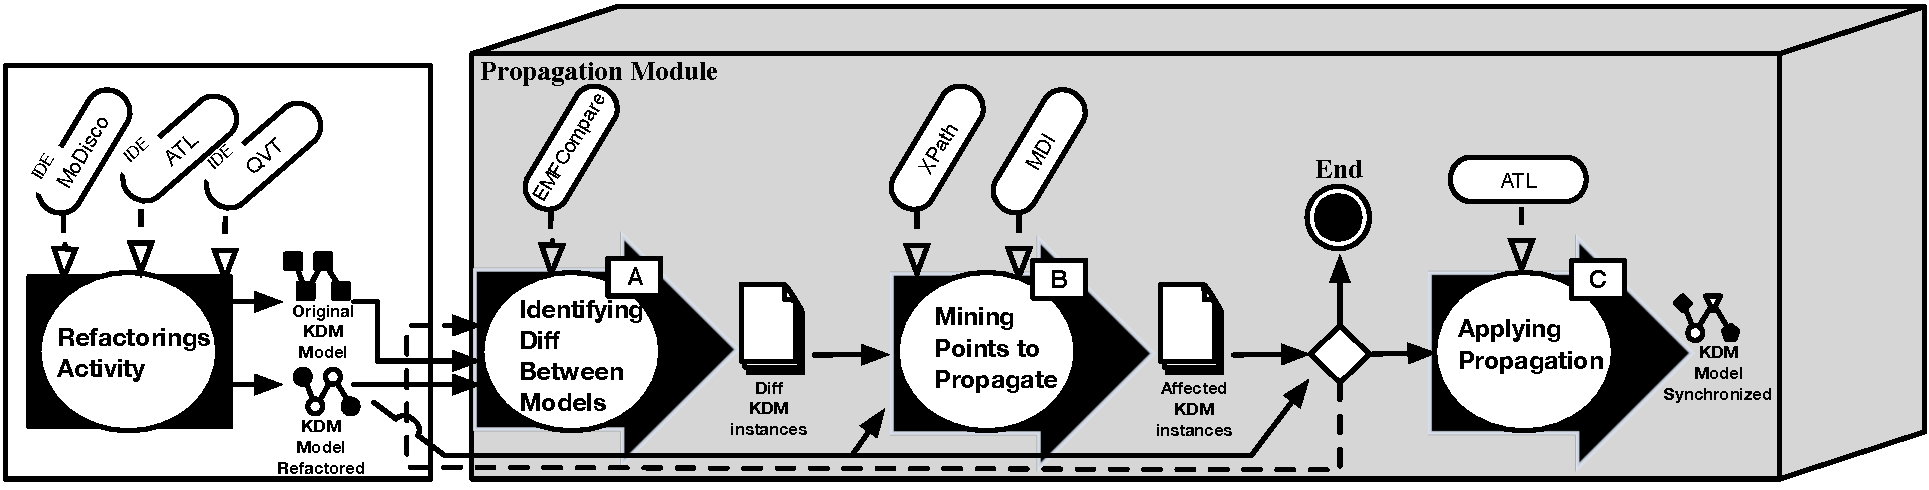
\includegraphics[scale=0.5]{images/ApproachLifeCicle2}
	\fautor
\end{figure}

Após a aplicação de um conjunto de refatorações o passo [A] pode ser iniciado. 

\section{Considerações Finais}
